% !TEX TS-program = xelatex
% !BIB TS-program = biber
% !TEX encoding = UTF-8 Unicode
%TC:macro \autocite [ignore]
%TC:macro \autocites 2 [ignore]

\documentclass[a4paper]{article}

\usepackage[bibstyle=apa,paper=a4paper]{../codes/latex/pccommon}
\usepackage{longtable}
\usepackage{titling}
\usepackage{listings}
\usepackage{abstract}
\usepackage{algorithm}
\usepackage{algpseudocode}

\begin{filecontents}{main.bib}
    @techreport{pcg2014,
    title = {{PCG}: A Family of Simple Fast Space-Efficient Statistically Good Algorithms for Random Number Generation},
    author = {Melissa E. O'Neill},
    institution = {Harvey Mudd College},
    address = {Claremont, CA},
    number = {HMC-CS-2014-0905},
    year = {2014},
    month = {9},
    url = {https://www.cs.hmc.edu/tr/hmc-cs-2014-0905.pdf},
    }
    @article{ieee754,
    author={},
    journal={IEEE Std 754-2019 (Revision of IEEE 754-2008)}, 
    title={{IEEE} Standard for Floating-Point Arithmetic}, 
    year={2019},
    volume={},
    number={},
    pages={1-84},
    doi={10.1109/IEEESTD.2019.8766229}}
    @techreport{iso9899,
    type = {Standard},
    key = {ISO/IEC 9899:1999},
    month = {12},
    year = {1999},
    title = {{Programming languages --- C}},
    address = {Geneva, CH},
    institution = {International Organization for Standardization}
    }
\end{filecontents}

\definecolor{codegreen}{rgb}{0,0.6,0}
\definecolor{codegray}{rgb}{0.5,0.5,0.5}
\definecolor{codepurple}{rgb}{0.58,0,0.82}
\definecolor{backcolour}{rgb}{0.95,0.95,0.92}

\lstdefinestyle{mystyle}{
    backgroundcolor=\color{backcolour},   
    commentstyle=\color{codegreen},
    keywordstyle=\color{magenta},
    numberstyle=\tiny\color{codegray},
    stringstyle=\color{codepurple},
    basicstyle=\ttfamily\footnotesize,
    breakatwhitespace=false,         
    breaklines=true,                 
    captionpos=b,                    
    keepspaces=true,                 
    numbers=left,                    
    numbersep=5pt,                  
    showspaces=false,                
    showstringspaces=false,
    showtabs=false,                  
    tabsize=2
}

\lstset{style=mystyle}

\title{Monte Carlo method to calculate areas: a series of attempts to optimize algorithms for a real-world problem}
\author{Maiyun Zhang}

\date{September 5, 2022}

\bibliography{main.bib}

% Print abstract in the title page
\renewcommand\maketitlehookd{
    \mbox{}\medskip\par
    \centering
    % Full-width abstract
    \begin{minipage}{0.8\textwidth}
        \begin{abstract}
            This essay presents a Monte Carlo-based method to calculate the area of a shape and several attempts to refine and optimize the algorithm. Through
            analyses based on the nature of the computational hardware and the algorithms, we are able to reduce the run time of the na\"\i{}ve method by more than 80 percent while still converging to the correct result.
            the nature of the computational hardware.
        \end{abstract}
        {\small\textit{Keywords:} Monte Carlo, optimization, integration}
    \end{minipage}
}

\begin{document}
\begin{titlepage}
    \LARGE
    \vspace*{\fill}
    \renewcommand{\arraystretch}{2}
    \centering
    \begin{tabular}{r@{:\,}p{0.6\columnwidth}}
    \textbf{Author} & Maiyun Zhang\\
    \textbf{Affiliation} & Pearson College UWC, Victoria, BC V9C 4H7, Canada\\
    \textbf{Instructor} & Mark Wheen\\
    \textbf{Title} & \makeatletter{}\@title{}\makeatother{}\\
    \textbf{Date of Submission} & \makeatletter{}\@date{}\makeatother{}
    \end{tabular}
    \vspace*{\fill}
\end{titlepage}
\begin{titlepage}
    \maketitle
    % Abstract handled by \maketitlehookd
    \tableofcontents
\end{titlepage}

\section{Introduction}
Monte Carlo methods use random sampling within a given sample space to numerically approximate the real result. With a proper random sampling method, they can approach the real result as the number of trials is increased. Therefore, they are often used on problems when it is non-trivial or even impossible to figure out the solution in closed form. Those methods have a wide range of applications from a computational simulation of complex systems to the calculation of the integral of a simple function.

Finding the area between curves is a traditional mathematical problem with varying degrees of difficulty from being elementary to being impossible. One question is formulated as such: A square has an inscribed circle of radius \(r\). Another circle's center is the lower right vertex of the square, and its radius is \(2r\). The two circles intersect at two points. What is the smaller area between the two circles (shown in Figure~\ref{fig:question}, the specified area is in gray) when \(r = 5\)?

\begin{figure}[hp]
\centering
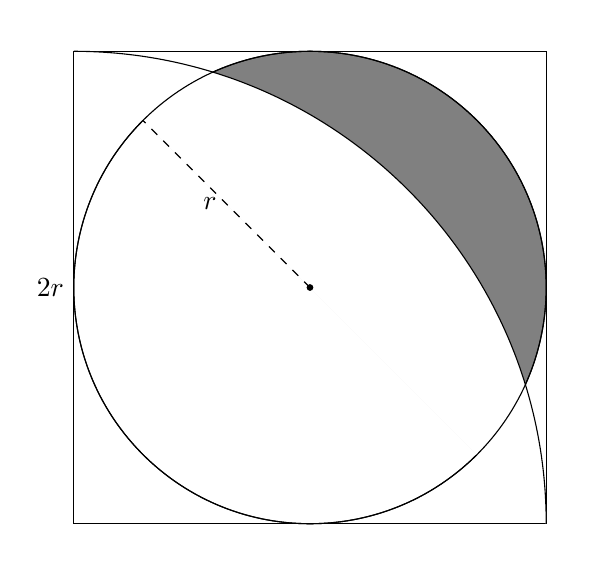
\begin{tikzpicture}
    \coordinate (UL) at (2.1213203435596424, -2.1213203435596424);
    \coordinate (LR) at (-2.1213203435596424, 2.1213203435596424);
    % Square
    \draw (-3, -3) -- node[anchor=east] {\(2r\)} (-3, 3) -- (3, 3) -- (3, -3) -- cycle;
    % Gray part
    \draw[fill=gray] (UL) arc(-45:135:3);
    % White part
    \draw (LR) arc(135:315:3);
    % Fix a gray area
    \draw[white] (UL) -- (LR);
    % Big arc, white
    \draw[fill=white] (3, -3) arc(0:90:6);
    % Fix the circle
    \draw (0, 0) circle (3);
    \filldraw (0,0) circle (1pt);
    \draw[dashed] (0, 0) -- node[anchor=east] {\(r\)} (LR);
\end{tikzpicture}
\caption{Diagram of the question}\label{fig:question}
\end{figure}

It is possible to use trigonometry to work out the area mathematically as shown in~\eqref{eq:real}, which evaluates to approximately \(S_\text{correct} = 14.638126\) with \(r = 5\). However, in this essay, we will examine a way to find the answer with Monte Carlo methods and optimize the method.

\begin{align}\label{eq:real}
    \frac{S}{r^2} &=
        \pi - \arccos\cfrac{-\sqrt{2}}{4} 
            - 4\arccos\cfrac{5\sqrt{2}}{8}
            + 2\sin\left(2\arccos\frac{5\sqrt{2}}{8}\right)
            - \frac{1}{2}\sin\left(
                2\pi - 2\arccos\frac{-\sqrt{2}}{4}
            \right) \notag \\
    &= \pi - \arccos -\frac{\sqrt{2}}{4}
        - 4 \arccos\frac{5\sqrt{2}}{8}
        + \frac{\sqrt{7}}{2}
\end{align}

\section{Equipments}
All the computations mentioned in this essay are completed on a MacBook Pro with an M1 chip running macOS 12.5.1. The C source files are compiled with LLVM clang version 14.0.6. The optimization flag is \textbf{-O3}.

\section{General Algorithm}
The overall process of performing this Monte Carlo experiment is as follows:
\begin{enumerate}
    \item Construct a Cartesian coordinate system: the lower left corner of the square in the question is the origin and the verticle side is the positive \(y\) direction.
    \item\label{step:gen} Generate a random point \((x, y)\) where \(x, y \in [0, 2r]\).
    \item\label{step:verify} Check if the generated random point lies inside the specified area.
    \item\label{step:incr} Increment the counter of points if that random point is in the specified area.
    \item Go back to Step~\ref{step:gen} for a given amount of random trials.
    \item Calculate the fraction of the random points which are in the specified area, then multiply it with the total area to get the result.
\end{enumerate}

With some pseudocode, the above algorithm can be more precisely described as shown in Algorithm~\ref{alg:gen}.

\begin{algorithm}
    \caption{General algorithm}\label{alg:gen}
    \begin{algorithmic}[1]
        \Procedure{GetArea}{\(r, n_\text{sample}\){}}
            \State{} \(n_\text{inside} \gets 0\) \Comment{Number of points inside the area}
            \State{}
            \Repeat{}
                \State{} \(x, y \gets \Call{GetRandPoint}{}\)
                \If{\Call{InArea}{\(x, y, r\){}}}
                    \State{} \(n_\text{inside} \gets n_\text{inside} + 1\)
                \EndIf{}
            \Until{\(n_\text{sample}\) trials are completed}
            \State\Return{\(4 r^2 \cfrac{n_\text{inside}}{n_\text{sample}} \){}}
        \EndProcedure{}
    \end{algorithmic}
\end{algorithm}

For the purpose of this project, we will only work on implementing and improving Step~\ref{step:verify}. For Step~\ref{step:gen}, we use the permuted congruential generator considering its speed and statistical idealness \autocite{pcg2014}. While this general method is relatively straightforward, there are various adjustments and optimizations that can be done to obtain an optimal version.

\section{Process}
\subsection{Initial Approach}
A rather standard way to compute the given result is by simply writing the standard equation of the two circles and using a Monte Carlo simulation to calculate the definite integral. There are three curves of concern on the graph:
\begin{enumerate}
    \item The upper half of the small circle:
        \begin{align}\label{eq:uh}
            {(y - r)} ^ 2 + {(x - r)} ^ 2 &= r ^ 2 \notag \\
            y_{1u} &= r + \sqrt{2 x r - x^2}
        \end{align}
    \item The lower half of the small circle:
        \begin{align}\label{eq:lh}
            {(y - r)} ^ 2 + {(x - r)} ^ 2 &= r ^ 2 \notag \\
            y_{1l} &= r - \sqrt{2 x r - x^2}
        \end{align}
    \item The large arc:
        \begin{align}\label{eq:la}
            y ^ 2 + x ^ 2 &= {(2r)} ^ 2 \notag \\
            y_2 &= r + \sqrt{4 r ^ 2 - x^2}
        \end{align}
\end{enumerate}

Looking at the graph, we can see that there are two parts to be considered: the area on the left is between the large arc and the circle, while the area on the right is between two halves of the small circle. The boundary can be found by solving~\eqref{eq:lh} and~\eqref{eq:la}:
\begin{align*}
    \begin{cases}
        x_b &= r \cfrac{5 + \sqrt{7}}{4},\\
        y_b &= r \cfrac{5 - \sqrt{7}}{4}
    \end{cases}
\end{align*}

Therefore, as shown in Algorithm~\ref{alg:chkfunc}, if the random point lies to the left of \(x_b\), we decide whether it is within the boundary by checking if \(y_2 \le x < y_{1u}\). Otherwise, we check if \(y_{1l} \le x < y_{1u}\).

\begin{algorithm}[hp]
    \caption{Point checking based on standard equation}\label{alg:chkfunc}
    \begin{algorithmic}[1]
        \Procedure{InArea}{\(x, y, r\){}}
            \If{\(x \le x_b\) \textbf{and} \(y_2 \le y < y_{1u}\){}}
                \State\Return{\textbf{true}}
            \ElsIf{\(x > x_b\) \textbf{and} \(y_{1l} \le y < y_{1u}\){}}
                \State\Return{\textbf{true}}
            \EndIf{}\\
            \State\Return{\textbf{false}}
        \EndProcedure{}
    \end{algorithmic}
\end{algorithm}

Shown in Algorithm~\ref{alg:chkfuncc} is a sample implementation of Algorithm~\ref{alg:gen} and~\ref{alg:chkfunc} in the C programming language. It uses the PCG32 generator to generate a random coordinate \((x, y) \in {[0, \text{UINT32\_MAX}]}^2\).

\begin{algorithm}[hp]
    \caption{Point checking based on standard equation --- C implementation}\label{alg:chkfuncc}
    \begin{lstlisting}[language=C]
uint64_t monte_carlo(const float radius, const uint64_t rand_samples)
{
    const float rmax = 2 * radius + 1;
    uint64_t i;
    uint64_t inside = 0;
    float x_dot, y_dot;
    float yu, yl, yt;
    pcg32_random_t rngx, rngy;
    pcg32_srand(&rngx, UINT64_C(42), UINT64_C(430));
    pcg32_srand(&rngy, UINT64_C(42), UINT64_C(431));

    for (i = 0; i < rand_samples; ++i)
    {
        x_dot = rmax * pcg32_rand(&rngx) / UINT32_MAX;
        y_dot = rmax * pcg32_rand(&rngy) / UINT32_MAX;
        yu = y1_upper(x_dot, radius);
        yl = y1_lower(x_dot, radius);
        yt = y2(x_dot, radius);
        /* left segment */
        if (radius * (5 - sqrt(7)) / 4.0 <= x_dot && x_dot < radius * (5 + sqrt(7)) / 4.0 &&
                 yt <= y_dot && y_dot < yu)
            ++inside;
        /* right segment */
        else if (radius * (5 + sqrt(7)) / 4.0 <= x_dot && yl <= y_dot && y_dot < yu)
            ++inside;
    }
    return inside;
}
    \end{lstlisting}
\end{algorithm}

\subsection{Evaluation of the Initial Approach}
When \(r = 5\) and with \(1.28\times 10^9\) random samples, the program gives \(n_\text{inside} = 154869079\), which means the estimated area is \(12.0991\). Compared to the correct result as calculated in~\eqref{eq:real}, only the first decimal digit is correct. There is a \(\cfrac{12.0991 - S_\text{correct}}{S_\text{correct}} = 17\% \) error.

The reason why the error from this approach is large is related to the nature of the hardware. The problem is that although \textbf{float} is intended to represent a real number, it is not able to distinguish all possible real numbers because a digital computer is discrete in its means of operation.
For example, modern computers use the IEEE754 format to store real numbers. In our coordinate range, \([0, 10]\), there are only approximately \(2^{30}\approx10^9\) different possible floats \autocite{ieee754}. Although the random generator can theoretically generate \(2^{32}\) different random integers uniformly, when we downsample the numbers to the given range, some possible sample values are lost. As a result, the accuracy cannot continue to increase after saturating the sample space.

\subsection{Scaling Factor}
Intuitively, we need to attempt to fully utilize the entire possible range of \textbf{float} numbers in order to maximize accuracy. For example, if we define
\begin{lstlisting}[language=C]
    const float rscaled = radius * rand_samples;
\end{lstlisting}
and then, we generate random coordinates in this upscaled range:
\begin{lstlisting}[language=C]
    const float rmax = 2 * rscaled + 1;
    x_dot = rmax * pcg32_rand(&thrd_rngx) / UINT32_MAX;
    y_dot = rmax * pcg32_rand(&thrd_rngy) / UINT32_MAX;
\end{lstlisting}

With the introduction of the scaling factor, the accuracy improves dramatically with the same amount of random samples. In this case, \(n\text{inside} = 187344347\), which gives an estimated area of \(14.6363\). Now the error decreases to only \(\cfrac{14.6363 - S_\text{correct}}{S_\text{correct}} = 0.013\% \).

\subsection{Optimization --- Constant Factoring}
Now that the algorithms produce consistent results, it is of our interest to optimize the code so that it takes less time to complete the simulation. One of the first things we can do is factor out the constants from the \textbf{for} loops. Three of the major constants that we identified are the scale for the random number generator and the two boundaries:
\begin{lstlisting}[language=C]
    const float scale = ldexp(rmax, -32);
    const float q5msqrt7 = (5 - sqrt(7)) / 4.0, q5asqrt7 = (5 + sqrt(7)) / 4.0;
    const float rq5msqrt7 = r * q5msqrt7, rq5asqrt7 = r * q5asqrt7;
\end{lstlisting}
Thus, in each iteration of the loop body, there is a lower number of floating point operations needed, and it therefore saves time.

\subsection{Optimization --- New Algorithm}
A problem with the current approach is that using the standard equations requires calculating multiple floating point square roots. Although a lot of the modern processors offer \textbf{sqrt} as an instruction, it is still one of the most time-consuming operations in the simulation. However, mathematically, it is not trivial to further reduce the number of floating point operations.

To further optimize the program, we need another way to implement Step~\ref{step:verify} that checks if a point lies in the specified area. Fortunately, we know that if a point lies in a circle, the distance from the center of the circle to the point must be less than the radius of the circle. Using this property, we propose an improved version of Algorithm~\ref{alg:chkfunc} in Algorithm~\ref{alg:chkhypot}: if the point is outside the big arc but inside the small circle, count it.

\begin{algorithm}[hp]
    \caption{Point checking based on the length of the hypotenuse}\label{alg:chkhypot}
    \begin{algorithmic}[1]
        \Procedure{InArea}{\(x, y, r\){}}
            \State{} \((x_\text{center}, y_\text{center}) \gets (r, r)\)
            \If{distance between \((x, y)\) and \((0, 0) \ge 2r\) \textbf{and} distance between \((x, y)\) and \((x_\text{center}, y_\text{center}) < r\)}
                \State\Return{\textbf{true}}
            \EndIf{}\\
            \State\Return{\textbf{false}}
        \EndProcedure{}
    \end{algorithmic}
\end{algorithm}

While the standard C library offers a \textbf{hypot} function that calculates the distance between two points, its main aim is to prevent overflow instead of to be fast \autocite{iso9899}. Therefore, in the program, we manually calculate \(\sqrt{{(\Delta x)}^2 + {(\Delta y)}^2}\) instead of invoking \textbf{hypot}. Now the body of the loop becomes:
\begin{lstlisting}[language=C]
    x_dot = pcg32_rand(&thrd_rngx) * scale;
    y_dot = pcg32_rand(&thrd_rngy) * scale;
    d1 = sqrt((r - x_dot) * (r - x_dot) + (r - y_dot) * (r - y_dot));
    d2 = sqrt(x_dot * x_dot + y_dot * y_dot);
    if (d1 < r && d2 >= 2 * r)
        ++inside;
\end{lstlisting}

\subsection{Optimization --- Removing Square Roots}
There is still another piece of optimization to complete: it is now possible to completely remove the use of \textbf{sqrt} because in \([0, \infty]\), \(f(x) = x^2\) is monotonic. Therefore, we only need to compare \(d^2\) and \(r^2\) and there is no need to take the square root.
\begin{lstlisting}[language=C]
    static inline float sqhypot(const float a, const float b)
    {
        return fma(a, a, b * b);
    }
\end{lstlisting}
And the loop body:
\begin{lstlisting}[language=C]
    x_dot = pcg32_rand(&thrd_rngx) * scale;
    y_dot = pcg32_rand(&thrd_rngy) * scale;
    sqd1 = sqhypot(r - x_dot, r - y_dot);
    sqd2 = sqhypot(x_dot, y_dot);
    if (sqd1 < sqr && sqd2 >= 4 * sqr)
        ++inside;
\end{lstlisting}

\section{Conclusion and Evaluation}
The run time (clock time) of all the programs is summarized in Table~\ref{tbl:rt}.
\begin{ctpt}
    \caption{Run Time (average of three)}\label{tbl:rt}
    \begin{tabular}{cc}
        \toprule
        Program & Clock time \\
        \midrule
        Initial Approach & \(\SI{13.72}{\second}\) \\
        Scaled & \(\SI{13.38}{\second}\) \\
        Fine Tuned & \(\SI{12.08}{\second}\) \\
        Initial Hypot & \(\SI{10.33}{\second}\) \\
        Fine Tuned & \(\SI{2.05}{\second}\) \\
        \bottomrule
    \end{tabular}
\end{ctpt}

It is clear that all the approaches reduced the time required to run this Monte Carlo algorithm. Even with compiler optimizations turned on, some small tweaks can still produce visible improvement. What this result suggests is that for critical pieces of code, it is worth it to improve its efficiency manually.

Simultaneously, the previous adjustments did not produce any significant improvement, while changing the algorithm instantly reduced more run time than all the previous attempts. Finally, an improvement to the most heavily-used routine provided an improvement of about \(80\% \). It suggests that while engineering algorithms, we should not focus on premature optimization, but rather work to improve the algorithm itself. 

\section{Acknowledgement}
May I express my gratitude to my instructor, Mark, who supported my exploration along the way.

Thank my parents for providing me with a perfect environment to learn and explore the world of computing.

\printbibliography{}

\end{document}
